\section{Introduction}
\label{sec:introduction}

\ac{pacs} are used to restrict access to physical areas, with most implementation relying on traditional authentication methods such as \ac{rfid} key cards or \ac{pin} codes.
While effective in enforcing basic access policies, these approaches suffer from several limitations, including their reliance on physical or intangible credentials that can be lost, stolen, or forgotten.
The lack of usability and convenience for end users --- constantly needing to carry a single-purpose physical token, and interact with an access control panel, for example --- leaves much to be desired.

Biometric authentication has grown in popularity in recent years, including within \ac{pacs} deployments.
This type of authentication enables use of inherence-factor-based identification methods like fingerprint, iris, and facial recognition.
Although these introduce a significant improvement to security by tying credentials to individual's physiology, most still require active participation and physical interaction with some form of access control interface.
Additionally, bias-related challenges, such as unbalanced facial recognition datasets leading to people (especially women) of darker skin tone being misclassified up to 'thirty-five times or more higher' than their white male counterparts, have raised ethical concerns regarding the use of biometric recognition technologies overall.

This project explores the use of \ac{gr} as a lesser-used biometric for access control.
By assessing the way a person walks --- a behavioural biometric --- the aim is to enable transparent, contactless authentication that maintains security without disrupting user flow.
\ac{gr} presents an opportunity to reduce friction for \ac{pacs} users while mitigating the risks associated with token-based systems and more obtrusive or intrusive biometric modalities.

To evaluate this approach, a prototype \ac{pacs} was developed that uses \ac{cv} to extract movement information from live video input.
This data is abstracted into a \ac{gei} --- representing statistical and spatio-temporal features of a subject's gait --- which is used to enable classification and identity verification.
The system follows a client-server architecture where the client is a lightweight application responsible for capturing video input and abstracting it into a gait cycle representation, while the server is responsible for gait sample storage, classification, and authorisation rule management.
The resulting solution aims to demonstrate the feasibility of \ac{gr}-based authentication and its potential for real-world use to enable secure, unobtrusive physical access control.

The proposed \ac{gr}-based access control system can be described as enabling 'pseudo-transparent authentication', providing an authentication mechanism that operates passively and is not immediately apparent to the user, but continues to maintain security by only permitting access to authorised individuals.

\subsection{Aims and Objectives}
\label{subsec:aims-and-objectives}

As defined above, this project aims to deliver a prototype access control system that uses \ac{gr} to passively identify subjects, in an attempt demonstrate the feasibility of assessing gait to perform authentication.
A distributed architecture is targeted, with a central application responsible for identification, receiving movement data input from a connected client or clients.
The idea is that future development could introduce support for multiple similtaneous clients, enabling gait-based authentication to be implemented across a site.

Figure \ref{fig:system-topology} below provides an overview of the desired system architecture, made up of two main components: (a) the \ac{acc} that captures movement data using \ac{cv} techniques, sending gait data to (b) the \ac{grs}, which assesses the input and returns the associated identity.
After receiving the identity prediction result and associated access control rule for the given input.
The \ac{acc} will evaluate this information to determine if access should be granted.

\begin{figure}[H]
    \centering
    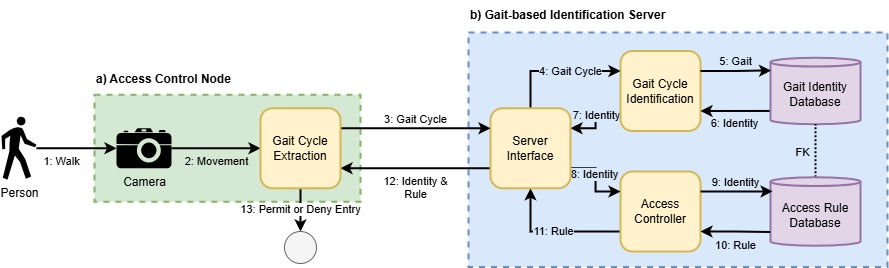
\includegraphics[width=0.9\textwidth]{assets/topology_diagram2.jpg}
    \caption{Gait Recognition-based Access Control System Topology }
    \label{fig:system-topology}
\end{figure}

\paragraph{\ac{gr}-based Identification} This \textit{could} be achieved using  \ac{ml} to evaluate gait cycle data, or simpler methods of similarity measurement.
As discussed in Chapter \ref{chap:context}, classification models can be trained on historic data, enabling subsequent identification of individuals from real-time (or historic) footage.
Alternatively, \ac{poc} could be achieved using simpler forms of similarity measurement like \ac{pda}, model-free \ac{nn} classification, or cosine similarity to assess similarities between input and historic data directly.
However, this is likely to be less effective than \ac{ml} model-based approaches, but may still enable demonstration of \ac{gr} as a \ac{poc}.

\paragraph{Access Control System Integration} \ac{cv}-based \ac{gr} is widely researched but is yet to see widespread adoption in real-world scenarios.
The \ac{acc} component would leverage the aforementioned \ac{grs} to demonstrate authentication, illustrating how it could be used in a \ac{pacs} context.
As shown in Figure \ref{fig:system-topology} above, movement data would be captured by the \ac{acc} and transmitted to the \ac{grs}, access would then be granted or denied in respect to a Boolean rule associated with the identity, mimicking how traditional \ac{pacs} operate (see Section \ref{subsec:overview-of-physical-access-control}).

Meeting these aims will require several objectives to be met, some of which are dependent on the prior completion of others.
Table \ref{tab:project-objectives} below outlines five (5) primary objectives of this project and specifies related dependencies.

\begin{scriptsize}
    \begin{longtable}[c]{|p{0.03\textwidth}|p{0.7\textwidth}|p{0.17\textwidth}|}
        \caption{Project Objectives}
        \label{tab:project-objectives}                                                                                                                                                                                                                                                                                                                                                 \\
        \hline
        \textbf{\#} & \textbf{Objective}                                                                                                                                                                                                                                                                                                                       & \textbf{Dependencies} \\ \hline
        \endfirsthead
        \caption*{Project Objectives (Continued)}                                                                                                                                                                                                                                                                                                                                      \\
        \hline
        \textbf{\#} & \textbf{Objective}                                                                                                                                                                                                                                                                                                                       & \textbf{Dependencies} \\ \hline
        \endhead
        \hline
        \endfoot
        1           & \textbf{Produce a prototype \ac{cv}-based gait identification system.} \par It should accept movement data as input and return an associated identity if found (e.g., matching with a previously registered identity).                                                                                                                   &                       \\
        2           & \textbf{Produce a prototype \ac{acc} that leverages the gait-based identification system.} \par The \ac{acc} should leverage the result of \#1 to enable identity authentication, allow for registration of new identities, support configuration of authorisation rules, and demonstrate provision or denial of access (as a \ac{poc}). & 1                     \\ \hline
        3           & \textbf{Test and evaluate the performance and accuracy of the gait-based identification.} \par The performance of \#1 and \#2 should be evaluated in order to determine performance and accuracy.                                                                                                                                        & 1                     \\ \hline
        4           & \textbf{Perform user testing (diverse subjects) and demonstrations to receive feedback and opinions.} \par Evaluate the final system to determine how well it meets initial goals and compares to other authentication methods in terms of usability. Address concerns and recommend improvements.                                       & 1, 2                  \\ \hline
        5           & \textbf{Evaluate the feasibility of implementing gait-based physical access control in the real-world.} \par Based on the results of \#3 and \#4, the feasibility of (\ac{cv}) \ac{gr}-based \ac{pacs} being implemented in the real-world should be discussed, alongside recommendations for further developments if necessary.         & 3, 4                  \\
    \end{longtable}
\end{scriptsize}

\subsection{Report Structure}
\label{sec:report-structure}

This report is structured into five chapters, each covering a different aspect of research, development, or evaluation:

\begin{itemize}
    \item \textbf{Chapter 1 --- Introduction:} Introduces the core problem area, the motivation behind the project, and the concept of \ac{gr} as a potential solution. The goals of the project are also outlined here.

    \item \textbf{Chapter 2 --- Context:} Provides an in-depth review of existing \ac{pacs} systems, authentication techniques, and the position of \ac{gr} within the broader scope of biometric authentication. Key issues with current techniques are discussed to justify the project's direction.

    \item \textbf{Chapter 3 --- New Ideas:} Outlines the proposed solution in detail, including system aims, objectives, and a breakdown of tasks to be completed. Implementation options are evaluated, a SWOT analysis is conducted, and planning is covered via requirement definitions, a Gantt chart, and test planning.

    \item \textbf{Chapter 4 --- Implementation:} Describes how the system was built, covering development methodology, tools, technologies, and the implementation of each component. This includes the gait cycle extraction logic, the \ac{acc}, the \ac{grs}, and the communication between them.

    \item \textbf{Chapter 5 --- Evaluation and Discussion:} Presents the results of functionality, performance, and user testing. Reflections on the effectiveness of the solution are provided, along with identified issues andlimitations and considerations for real-world use. The chapter ends with a discussion on future directions.
    
    \item \textbf{Chapter 6 --- Conclusion:} Summarises achievements and critisisms based on the outcome of the project, and provides recommendations for future work if improvements are to be made. Disusses pertinent Legal, Ethical, Social, and Professional issues, and concludes with a personal reflection..

\end{itemize}

Each chapter builds upon the last, gradually leading from concept to implementation and evaluation, with the aim of clearly demonstrating the feasibility of using \ac{gr}-based authentication for physical access control.
